\chapter{THEORETICAL BASIS}

\renewcommand{\headrulewidth}{0.5pt}
\renewcommand{\footrulewidth}{0.5pt}
\thispagestyle{plain}
\pagestyle{fancy}
\fancyhf{}
\fancyhead[L]{\textbf{CHAPTER 2}}
\fancyhead[R]{\textbf{DROWSINESS DETECTION AND ALERT SYSTEM IN THE CAR}}
\raggedright
\fancyfoot[L]{From: Nguyen Van Anh Tuan}
\fancyfoot[R]{Page \thepage}

\section{Overview About Image Processing}
    \subsection{Introduction about Image Processing}
        Image processing is a method to perform some operations on an image, 
        in order to get an enhanced image or to extract some useful information from it. It is a type of signal 
        processing in which input is an image and output may be image or characteristics/features associated with 
        that image. Nowadays, image processing is among rapidly growing technologies. It forms core research area 
        within engineering and computer science disciplines too. \\ 
        \vspace{3mm}
        Image processing basically includes the following 3 steps:
        \begin{itemize}
            \item Importing the image via image acquisition tools
            \item Analysing and manipulating the image
            \item Output in which result can be altered image or report that is based on image analysis
        \end{itemize}
        There are two types of methods used for image processing namely, analogue and digital image processing. 
        Analog image processing can be used for the hard copies like printouts and photographs. Image analysts use 
        various fundamentals of interpretation while using these visual techniques. Digital image processing techniques 
        help in manipulation of the digital images by using computers. The three general phases that all types of data 
        have to undergo while using digital technique are pre-processing, enhancement, and display, information extraction.
        \begin{figure}[H]
            \centering
            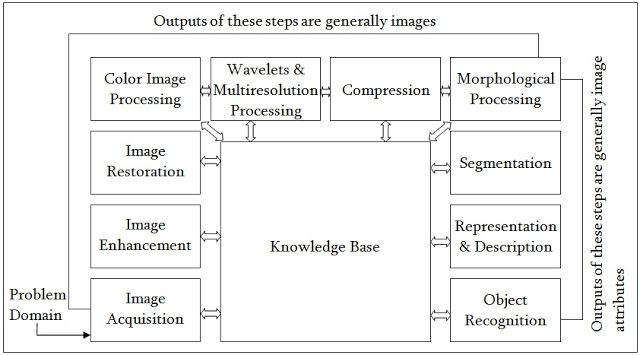
\includegraphics[width=0.6\linewidth]{img/IP.jpg}
            \caption{Fundamental steps in digital processing}
        \end{figure}
        \subsubsection{Image Acquistion}
            This is the first step or process of the fundamental steps of digital image processing. Image acquisition could 
            be as simple as being given an image that is already in digital form. Generally, the image acquisition stage involves 
            preprocessing, such as scaling etc.
        \subsubsection{Image Enhancement}
            Image enhancement is among the simplest and most appealing areas of digital image processing. Basically, the idea behind 
            enhancement techniques is to bring out detail that is obscured, or simply to highlight certain features of interest in an 
            image. Such as, changing brightness \& contrast etc.
        \subsubsection{Image Restoration}
            Image restoration is an area that also deals with improving the appearance of an image. However, unlike enhancement, 
            which is subjective, image restoration is objective, in the sense that restoration techniques tend to be based on mathematical 
            or probabilistic models of image degradation.
        \subsubsection{Color Image Processing}
            Color image processing is an area that has been gaining its importance because of the significant increase in the use of digital 
            images over the Internet. This may include color modeling and processing in a digital domain etc.
        \subsubsection{Wavelets and Multiresolution Processing}
            Wavelets are the foundation for representing images in various degrees of resolution. Images subdivision successively into smaller 
            regions for data compression and for pyramidal representation.
        \subsubsection{Compression}
            Compression deals with techniques for reducing the storage required to save an image or the bandwidth to transmit it. Particularly in 
            the uses of internet it is very much necessary to compress data.
        \subsubsection{Morphological Processing}
            Morphological processing deals with tools for extracting image components that are useful in the representation and description of shape.
        \subsubsection{Segmentation}
            Segmentation procedures partition an image into its constituent parts or objects. In general, autonomous segmentation is one of the most difficult 
            tasks in digital image processing. A rugged segmentation procedure brings the process a long way toward successful solution of imaging problems that 
            require objects to be identified individually.
        \subsubsection{Representation and Description}
            Representation and description almost always follow the output of a segmentation stage, which usually is raw pixel data, constituting either the boundary 
            of a region or all the points in the region itself. Choosing a representation is only part of the solution for transforming raw data into a form suitable 
            for subsequent computer processing. Description deals with extracting attributes that result in some quantitative information of interest or are basic for 
            differentiating one class of objects from another.
        \subsubsection{Object Recognition}
            Recognition is the process that assigns a label, such as, “vehicle” to an object based on its descriptors.
        \subsubsection{Knowledge Base}
            Knowledge may be as simple as detailing regions of an image where the information of interest is known to be located, thus limiting the search that has to be 
            conducted in seeking that information. The knowledge base also can be quite complex, such as an interrelated list of all major possible defects in a materials 
            inspection problem or an image database containing high-resolution satellite images of a region in connection with change-detection applications.
    \subsection{The Components of Image Processing}
        \subsubsection{Digital Image}
            A digital image is a finite set of pixels with a gray level suitable for describing an image close to the real image. The number of pixels 
            determines the resolution of the image. The higher quality of the image, the more clearly the image's points are displayed, making the image 
            more realistic and sharp.
        \subsubsection{Picture Element}
            In digital imaging, pixel, pel, or picture element is a smallest addressable element in a raster image, or the smallest addressable element in an \textbf{all points 
            addressable display device}; so it is the smallest controllable element of a picture represented on the screen. \\ 
            \vspace{3mm}
            Each pixel is a sample of an original image; more samples typically provide more accurate representations of the original. The intensity of each pixel is variable. 
            In color imaging systems, a color is typically represented by three or four component intensities such as red, green, and blue, or cyan, magenta, yellow, and black. \\ 
            \vspace{3mm}
            In some contexts (such as descriptions of \textbf{camera sensors}), pixel refers to a single scalar element of a multi-component representation (called a photosite in the 
            camera sensor context, although sensel is sometimes used), while in yet other contexts it may refer to the set of component intensities for a spatial position.
            \begin{figure}[H]
                \centering
                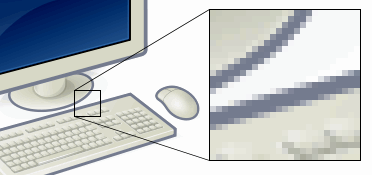
\includegraphics[width=0.6\linewidth]{img/Pixel-example.png}
                \caption{Pixel example}
            \end{figure}
            Pixel is an element of digital image at coordinate (x,y) with gray level or certain color. The size and the distance between those pixels are chosen appropriately so that 
            the human eye perceives spatial continuity and gray level (or color) of digital image like real image. Each of element in matrix is called an image element.
        \subsubsection{Gray Level of Picture}
            Gray level is the result of conversion of 1 luminosity value of 1 pixel positive integer value. Usually identified in [0,255] depending on the value each pixel is 
            represented. Common gray scale values is: 16, 32, 64, 128, 256 (level 256 is universal level). The reason is computer techniques use 1 byte (8 bits) to represent 
            the gray level. Gray level use 1 byte represent: 28 = level 256, it mean from 0 to 255).
            \begin{figure}[H]
                \centering
                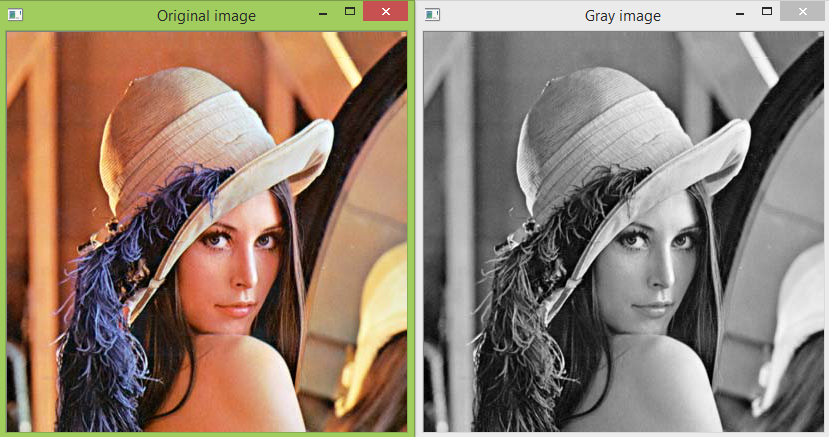
\includegraphics[width=0.6\linewidth]{img/gray-scale.png}
                \caption{Gray scale image example}
            \end{figure}
        \subsubsection{Image Resolution}
            Image resolution is detail an image holds. The term applies to raster digital images, film images, and other types of images. Higher resolution means more image detail. \\ 
            \vspace{3mm}
            Image resolution can be measured in various ways. Resolution quantifies how close lines can be to each other and still be visibly resolved. Resolution units can be tied 
            to physical sizes (e.g. lines per mm, lines per inch), to the overall size of a picture (lines per picture height, also knnown simply as lines, TV lines, or TVL), 
            or to angular subtense. Line pairs are often used instead of lines; a line pair comprises a dark line and an adjacent light line. A line is either a dark line or 
            a light line. A resolution of 10 lines per milimeter means 5 dark line alternating with 5 light lines, or 5 line pairs per milimeter (5 LP/mm). Photographic lens and film 
            resolution are most often quoted in line pairs per milimeter. \\ 
            \vspace{3mm}
            For example: Image resolution in CGA display (Color Graphic Adaptor) is a grid of points across the screen: 320 vertical points * 200 image points (320*200).
            Obviously, with the same CGA display 12 inches we notice smoother than the screen CGA 17 inches with resolution is 320*200. The reason is with the same resolution but 
            the larger the screen area, the less smooth.
        \subsubsection{Types of image classification}
            \begin{itemize}
                \item \textbf{Binary Image:} is one that consists of pixels that can have one of exactly two colors, usually black and white. Binary images are also called bi-level 
                or two-level, Pixelart made of two colours is often referred to as 1-Bit or 1bit. This means that each pixel is stored as a single bit—i.e., a 0 or 1. \\
                \vspace{2mm}
                The names black-and-white, B\&W, monochrome or monochromatic are often used for this concept, but may also designate any images that have only one sample per pixel, 
                such as grayscale images. In Photoshop parlance, a binary image is the same as an image in "Bitmap" mode. \\ 
                \vspace{2mm}
                Binary images often arise in digital image processing as masks or thresholding, and dithering. Some input/output devices, such as laser printers, fax machines, 
                and bilevel computer displays, can only handle bilevel images. \\ 
                \vspace{2mm}
                A binary image can be stored in memory as a bitmap, a packed array of bits. A 640×480 image requires 37.5 KiB of storage. Because of the small size of the image files, 
                fax machine and document management solutions usually use this format. Most binary images also compress well with simple run-length compression schemes. \\ 
                \vspace{2mm}
                Binary images can be interpreted as subsets of the two-dimensional integer lattice $Z^2$; the field of morphological image processing was largely inspired by this view.
                \item \textbf{RGB Image:} RGB Color Model is an additive color model, in which red, green, and blue light are added together in various ways to reproduce a broad array 
                of colors. The name of the model comes from the initials of the three additive primary colors, red, green, and blue. \\ 
                \vspace{2mm}
                RGB is a device-dependent color model: different devices detect or reproduce a given RGB value differently, since the color elements (such as phosphors or dyes) 
                and their response to the individual R, G, and B levels vary from manufacturer to manufacturer, or even in the same device over time. Thus an RGB value does not define 
                the same color across devices without some kind of color management.
                \begin{figure}[H]
                    \centering
                    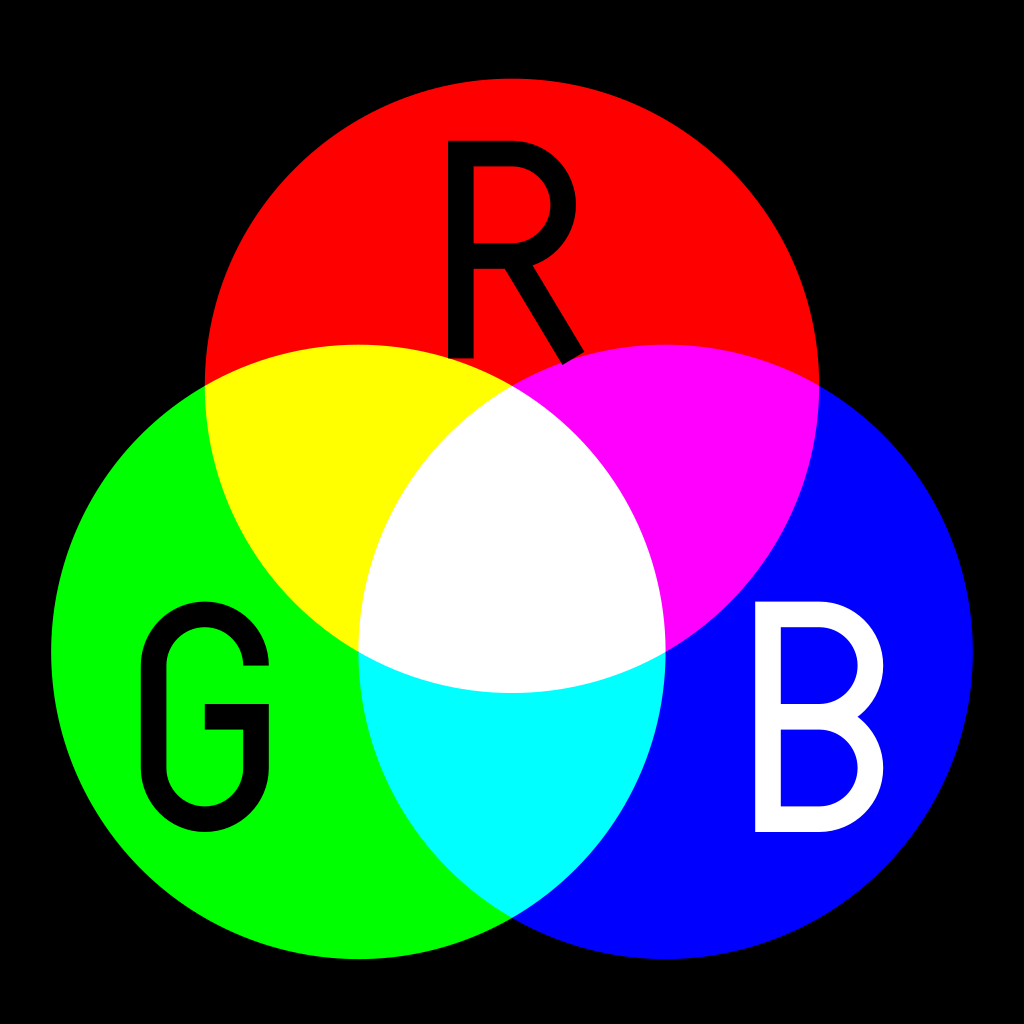
\includegraphics[width=0.6\linewidth]{img/RGB.png}
                    \caption{Additive color mixing}
                \end{figure}
                The choice of primary colors is related to the physiology of the human eye; good primaries are stimuli that maximize the difference between the responses of the cone 
                cells of the human retina to light of different wavelengths, and that thereby make a large color triangle. \\ 
                \vspace{2mm}
                The normal three kinds of light-sensitive photoreceptor cells in the human eye (cone cells) respond most to yellow (long wavelength or L), green (medium or M), 
                and violet (short or S) light (peak wavelengths near 570 nm, 540 nm and 440 nm, respectively). The difference in the signals received from the three kinds allows 
                the brain to differentiate a wide gamut of different colors, while being most sensitive (overall) to yellowish-green light and to differences between hues in the 
                green-to-orange region.
                \begin{figure}[H]
                    \centering
                    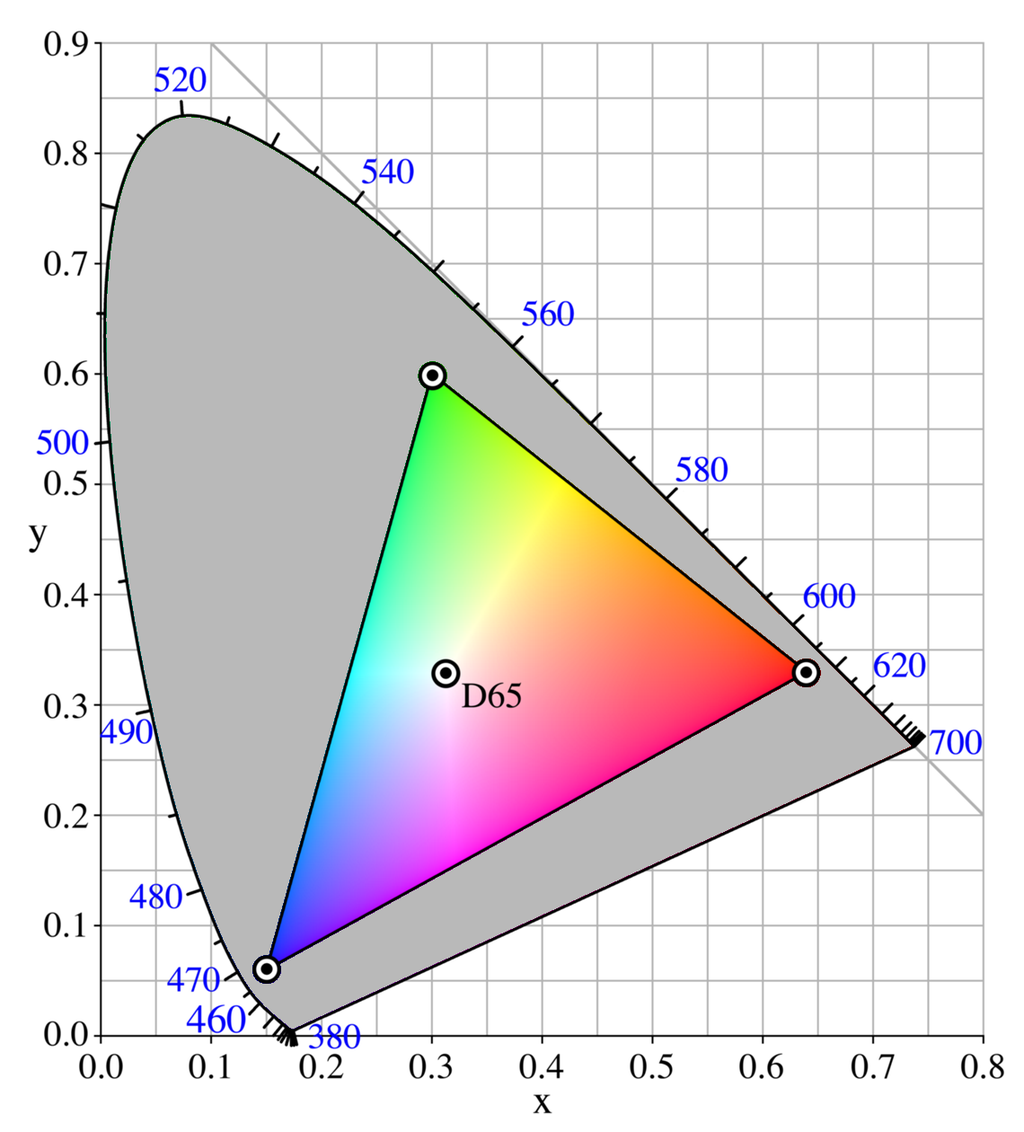
\includegraphics[width=0.6\linewidth]{img/primary-color.png}
                    \caption{A set of primary colors, such as the sRGB primaries, define a color triangle}
                \end{figure}
                \item \textbf{Image Transformation:} is a function. A function that maps one set to another set after performing some operations. \\ 
                \vspace{2mm}
                Image transformation is consider this equation:
                \begin{align}
                    G(x,y) = T{f(x,y)}
                \end{align}
                In this equation, $F(x,y)$ is input image on which transformation function has to be applied; $G(x,y)$ is the output image or processed image; $T$ is the transformation 
                function. This relation between input image and the processed output image can also be represented as: $s = T(r)$ where $r$ is actually the pixel value or gray level intensity 
                of $f(x,y)$ at any point. And $s$ is the pixel value or gray level intensity of $g(x,y)$ at any point. \\
                \vspace{2mm}
                The basic gray level transformation has been discussed in our tutorial of basic gray level transformations. There is some image transformations like: \texttt{Fourier Transform, Cousin, 
                Sin, convolution transform, Kronecker product}.
            \end{itemize}
    \subsection{Parts of The Image Processing System}
        \begin{figure}[H]
            \centering
            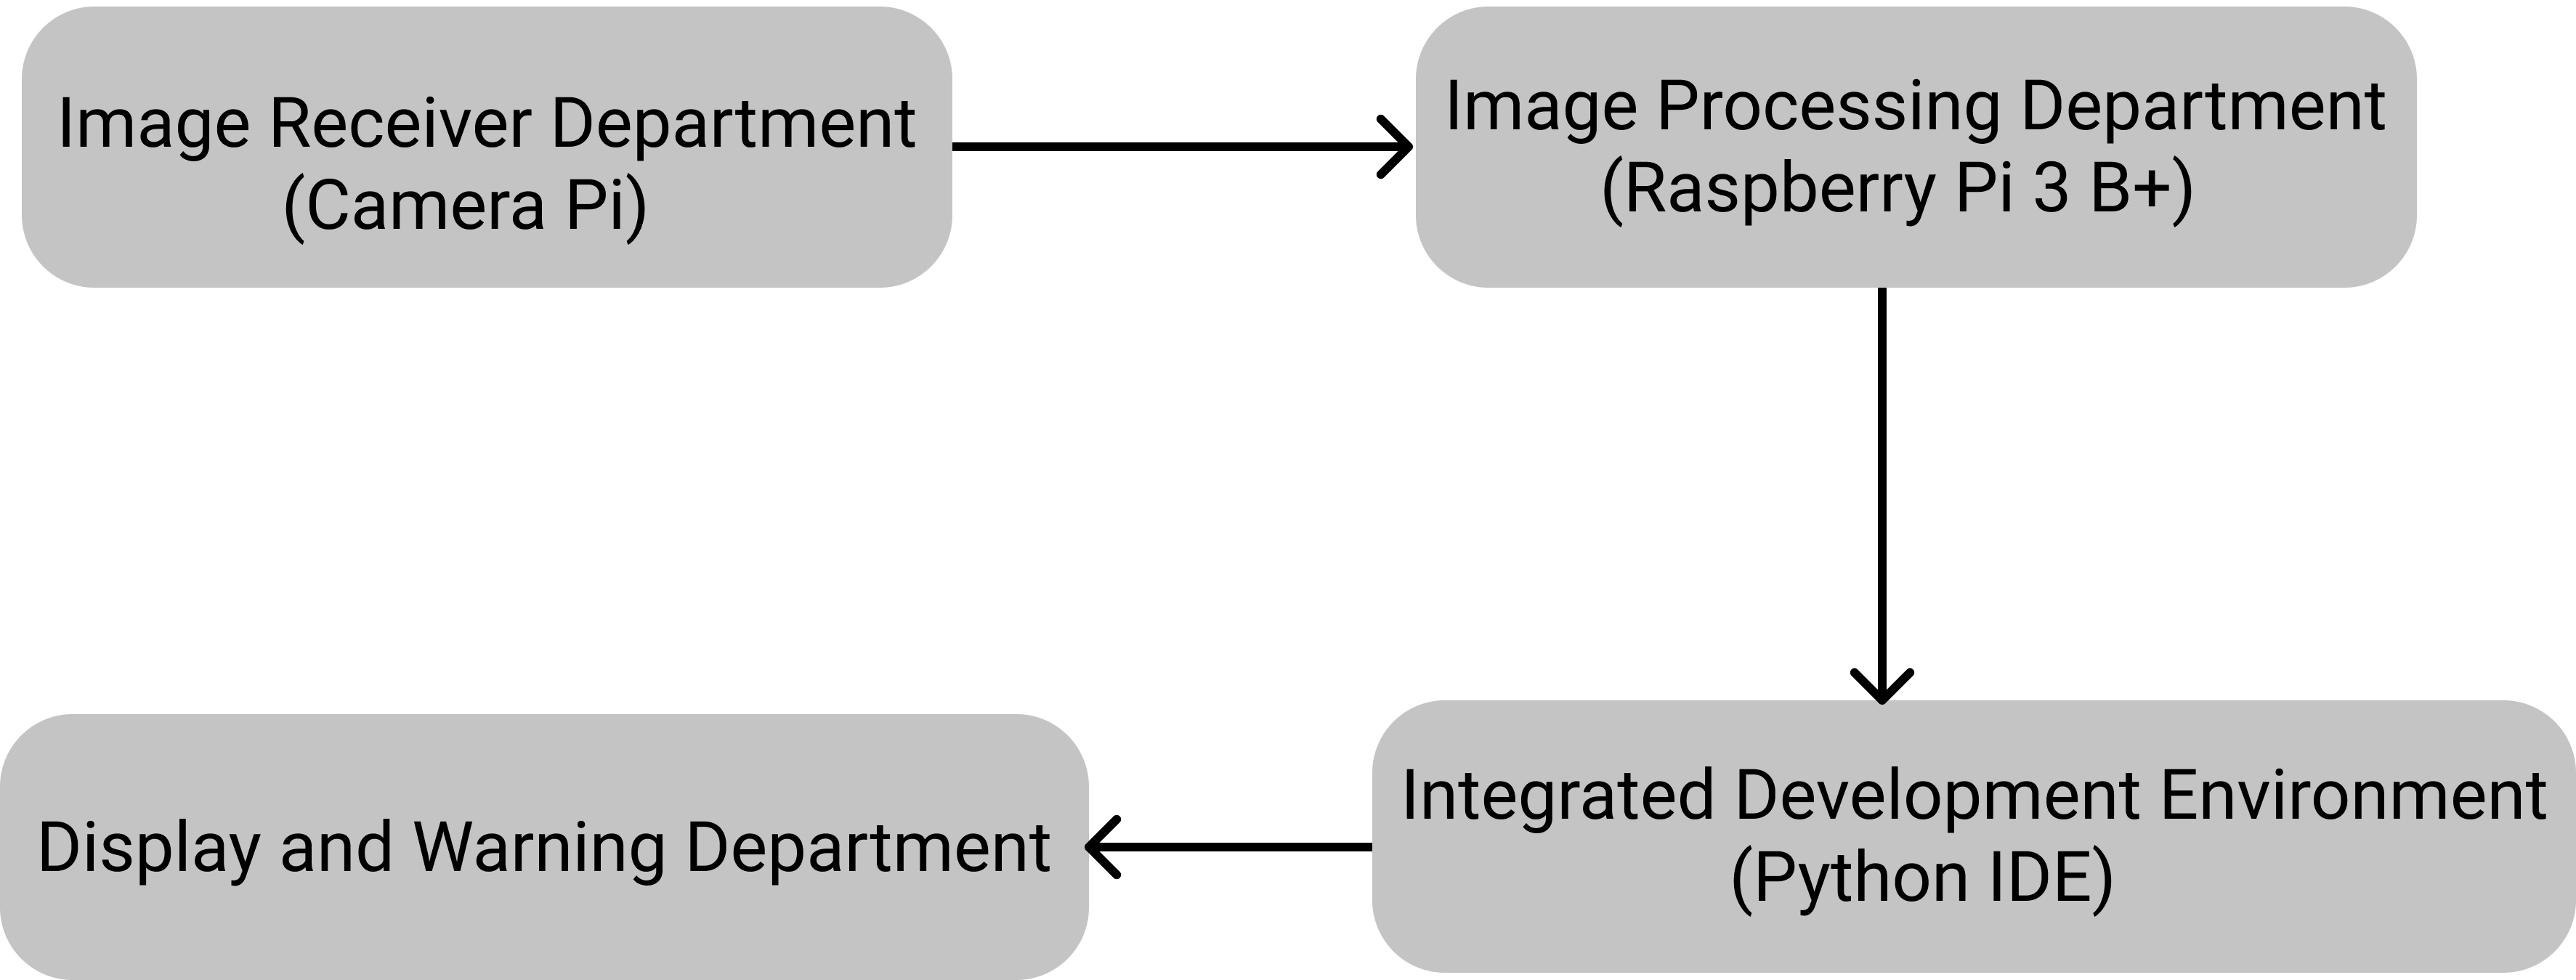
\includegraphics[width=0.6\linewidth]{img/Drowsiness.png}
            \caption{The part of image processing system}
        \end{figure}
        \textbf{Image Receiver Department} is usually a camera, scaners, image sensor,... In this project, a pi camera with 5mpx resolution is used to capture images. \\ 
        \vspace{3mm}
        \textbf{Image Processing Department} is specialized processing equipment or computers,... Specifically here using a Raspberry pi 3B + computer for image processing. \\ 
        \vspace{3mm}
        \textbf{Integrated Development Environment} using Thony Python IDE software to write program. \\ 
        \vspace{3mm}
        \textbf{Display and Warning Department} 7 inches for system operation and speaker alarms.

\section{Face Regconition Algorithm}

\section{Euclidean Distance}

\section{OpenCV}

\section{Python Programming Language}

\section{Introduction about Dlib}

\section{Raspberry Pi 3B +}